%FOR PDFLATEX USE ONLY
\documentclass[a4paper,12pt]{article}

\usepackage{amssymb,amsmath}

\usepackage[margin=2cm]{geometry}
\usepackage[unicode]{hyperref}
\usepackage[pdftex]{graphicx}
\usepackage{cmlgc}

\usepackage{array}

\usepackage{wrapfig}
\usepackage{array}
\usepackage{lipsum}
\usepackage{esvect}
\usepackage{hyperref}

\usepackage{subfig}
\usepackage{calc}
\usepackage{pgfplots,tikz,circuitikz}
\usepackage{pgfplotstable}
\usepackage{tkz-euclide}

\usepackage{centernot}
\usepackage{cancel}

\usepackage{mathtext}
\usepackage[T1,T2a]{fontenc}
\usepackage[utf8]{inputenc}
\usepackage[english, bulgarian, russian]{babel}
\usepackage{tikz}
\usepackage{pgfplots}
\usepackage[export]{adjustbox}
\usepackage[left=2cm,right=2cm,
    top=2cm,bottom=2cm,bindingoffset=0cm]{geometry}
\usepackage{indentfirst}
\usepackage{braket}
\usepackage{booktabs}

\begin{document}

\begin{center}
  \LARGE{Работа 2.5.1}\\[0.2cm]
  \LARGE{Измерение коэффициента поверхностногонатяжения жидкости!}\\[0.2cm]
  \large{Малиновский Владимир}\\[0.2cm]
  \normalsize{\texttt{galqiwi@galqiwi.ru}}
\end{center}

\textbf{Цель работы:} 1) измерение коэффициента поверхностного натяжения исследуемой жидкости при разной температуре с использованием известного коэффициента поверхностного натяжениядругой жидкости 2) определение полной поверхностной энергиии теплоты, необходимой для изотермического образования единицы поверхности жидкости.

\textbf{В работе используются:} прибор Ребиндера с термостатом, исследуемые жидкости, стаканы.

\section*{Описание работы}

Наличие поверхностного слоя приводит к различию давлений поразные стороны от искривленной границы раздела двух сред. Для сферического пузырька внутри жидкости избыточное давление дается формулой Лапласа
$$\Delta P = P_\text{внутри}-P_\text{снаружи}=2\sigma/r.$$
Эта формула лежит в основе предлагаемого метода определения коэффициента поверхностного натяжения жидкости. Измеряется давление, необходимое для выталкивания в жидкость пузырька газа.\\

Наличие поверхностного слоя приводит к различию давлений по разные стороны от искривленной границы раздела двух сред. Для сферического пузырька внутри жидкости избыточное давление дается формулой Лапласа $\Delta P = P_\text{внутри}-P_\text{снаружи}=2\sigma/r$. Эта формула лежит в основе предлагаемого метода определения коэффициента поверхностного натяжения жидкости. Измеряется давление, необходимое для выталкивания в жидкость пузырька газа.

Исследуемая жидкость наливается в сосуд $B$. Дистиллированная вода наливается в сосуд $E$. Сосуды закрыты пробками. Через пробку сосуда, в котором проводятся измерения, проходит полая металлическая игла $С$, нижний конец которой погружен в жидкость, а верхний открыт в атмосферу. Если другой сосуд герметично закрыт, то в сосуде с иглой создается разрежение, и пузырьки воздуха начинают пробулькивать через жидкость. Поверхностное натяжение можно найти по величине разрежения, необходимого для прохождения пузырьков. При приоткрытом кране $\text{К}_1$ из аспиратора $A$ по каплям вытекает вода, создавая разрежение, которое измеряется наклонным спиртовым манометром $М$. Показания манометра, умноженные на зависящий от наклона коэффициент ($0.2$), дают давление в $\text{кгс}/\text{м}^2$. Чтобы пополнить запас воды, достаточно при помощи крана $\text{К}_2$ соединить нижнюю часть аспиратора с атмосферой и предварительно заполненной водой верхней частью. Через рубашку $D$ непрерывно прогоняется вода из термостата для стабилизации температуры исследуемой жидкости.

\newpage
Схема установки представлена на рис. 1:
\begin{center}
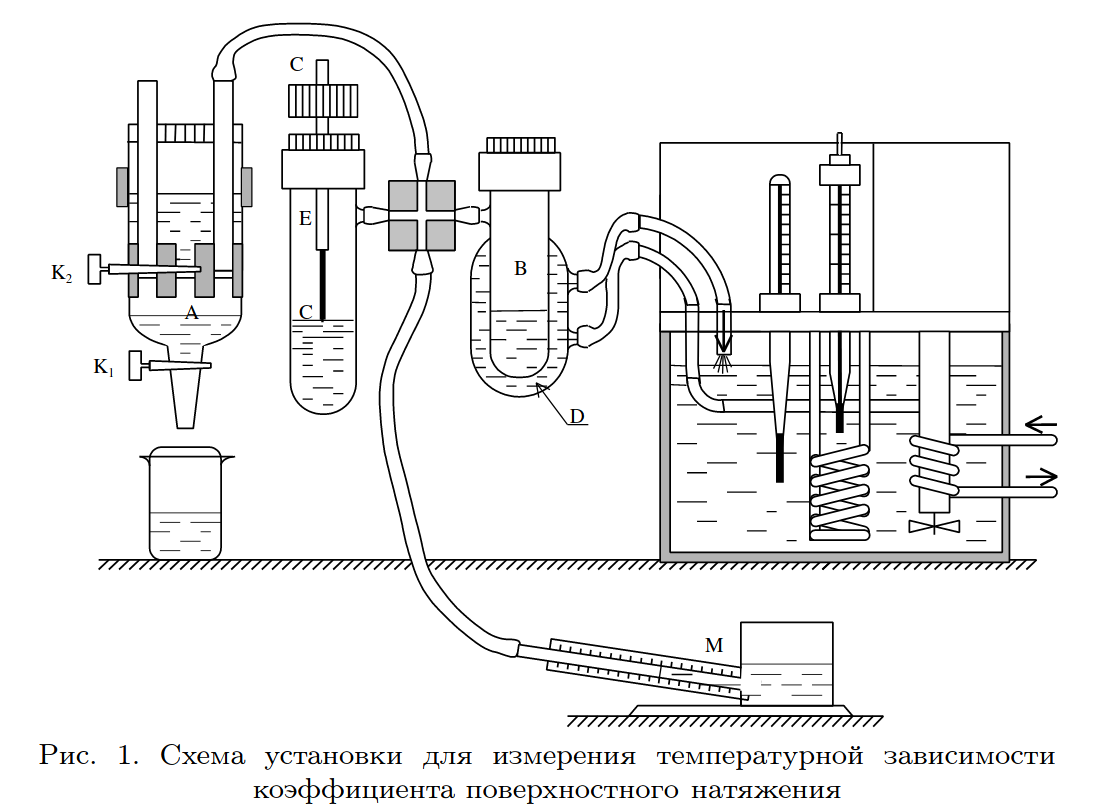
\includegraphics[width=0.95\textwidth]{equip.png}.
\end{center}
\newpage

В начале эксперимента зальем аспиратор $A$ водой, и поместим чистую иглу в сосуд со спиртом $B$ так, чтобы кончик иглы лишь касался поверхности.\\
Откроем кран $K_1$, в следствие этому давление в установке упадет, из-за чего показания манометра вырастут. Проверим установку на наличие утечки, закрыв кран $K_1$. Если показания манометра не меняются со временем, то все в порядке.\\
При открытом кране так, что период падения капель равна $\approx 5 \text{с}$, давление прекращает расти при значении, равном $2\sigma/(r\,\sin(\alpha))$, поскольку при нем образуется пузырек газа в шприце, и давление падает. На манометре получаются давления:\\

\begin{center}
\begin{tabular}{|c|c|c|c|c|c|c|c|c|c|c|c|c|c|c|c|c|}
\hline
$p,\,\text{кгс}/\text{м}^2$&$55$&$54$&$55$&$54$&$55$&$55$&$55$&$54$&$55$&$54$&$55$&$55$&$54$&$54$&$54$&$54$\\
\hline
\end{tabular},
\end{center}
$$\Delta p = 0.5\,\text{кгс}/\text{м}^2, \sin(\alpha) = 0.2.$$
Из измерений следует, что
$$p = (54.5 \pm 0.6) \text{кгс}/\text{м}^2.$$
Взяв табличное значение вязкости спитра $\sigma = (22\pm2) \text{мН}/\text{м}$, получим диаметр, равный
$$d_\text{косв} = \frac{4\sigma}{p\sin(\alpha)} = (0.82\pm0.08) \text{мм}.$$
Измерив диаметр иголки под микроскопом, получаем значение диаметра, равное
$$d_\text{прям} = (1.05\pm0.03) \text{мм}.$$
Промыв и просушив иглоку, переставим ее в сосуд с водой. Сначала измерим давления появления пузырьков при касании иголкой воды (при высоте иголки над дном сосуда $h_1$), а потом измерим то же самое, но при максимальном погружении иглы -- $h_2$.
\begin{center}
	\begin{tabular}{|c|c|c|c|c|c|c|c|}
	\hline
	$h,\,\text{мм}$ & \multicolumn{5}{c|}{$p,\,\text{кгс}/\text{м}^2$} & $<p>,\,\text{кгс}/\text{м}^2$ & $\Delta<p>,\,\text{кгс}/\text{м}^2$\\
	\hline
	$37.5$&$134$&$133$&$133$&$133$&$133$&$133.2$&$0.5$\\
	\hline
	$30.5$&$176$&$176$&$176$&$176$&$175$&$175.8$&$0.5$\\
	\hline
	\end{tabular}
\end{center}
$$\Delta h = 0.25\,\text{мм},\,\Delta p = 0.5\,\text{кгс}/\text{м}^2, \sin(\alpha) = 0.2.$$
Прямое измерение $h_1 - h_2$ дает результат:
$$h_1 - h_2 = 7 \pm 1 \text{мм}.$$
Из давлений следует, что разница высот:
$$\frac{p_2 - p_1}{\rho\,g}sin(\alpha)=8.5\pm0.2\text{мм}.$$
Далее проведем опыт при самой большой глубине погружения иглы и разной температуте. Для того, чтобы достичь равномерного прогрева воды в установке, после смены температуры термостата, подождем $5$ минут перед измерениями давления.
Результаты представлены ниже:
\begin{center}
\begin{tabular}{|c|c|c|c|c|c|c|c|c|c|c|c|c|c|c|c|}
\hline
$T,\,^\circ C$&\multicolumn{15}{c|}{$p,\,\text{кгс}/\text{м}^2$}\\
\hline
$23$&$176$&$176$&$176$&$176$&$175$&$--$&$--$&$--$&$--$&$--$&$--$&$--$&$--$&$--$&$--$\\
\hline
$30$&$174$&$174$&$175$&$175$&$174$&$175$&$--$&$--$&$--$&$--$&$--$&$--$&$--$&$--$&$--$\\
\hline
$35$&$174$&$174$&$174$&$174$&$174$&$174$&$173$&$173$&$174$&$174$&$174$&$174$&$174$&$173$&$174$\\
\hline
$40$&$172$&$172$&$172$&$172$&$172$&$172$&$172$&$172$&$172$&$172$&$172$&$172$&$172$&$172$&$172$\\
\hline
$45$&$171$&$171$&$171$&$171$&$171$&$171$&$171$&$171$&$171$&$171$&$171$&$171$&$171$&$171$&$171$\\
\hline
$50$&$170$&$170$&$169$&$169$&$170$&$170$&$170$&$169$&$169$&$170$&$170$&$169$&$170$&$170$&$170$\\
\hline
$55$&$169$&$169$&$169$&$169$&$169$&$169$&$169$&$170$&$170$&$169$&$169$&$170$&$170$&$169$&$169$\\
\hline
$60$&$168$&$169$&$168$&$168$&$168$&$168$&$168$&$168$&$169$&$169$&$168$&$168$&$168$&$168$&$168$\\
\hline
\end{tabular}
\end{center}
Из данных выше можно найти $<p>$ и $\sigma = \frac{pr}{2} \sin(\alpha)$.
\begin{center}
\begin{tabular}{|c|c|c|}
\hline
$T,\,^\circ C$&$<p>,\,\text{кгс}/\text{м}^2$&$\sigma, \text{мН}/\text{м}$\\\hline
$23.0$&$175.8$&$90$\\ \hline
$30.0$&$174.5$&$90$\\ \hline
$35.0$&$173.8$&$89$\\ \hline
$40.0$&$172.0$&$88$\\ \hline
$45.0$&$171.0$&$88$\\ \hline
$50.0$&$169.7$&$87$\\ \hline
$55.0$&$169.3$&$87$\\ \hline
$60.0$&$168.2$&$87$\\ \hline
\end{tabular}
\end{center}
$$\Delta p = \Delta <p> = 0.5\,\text{кгс}/\text{м}^2, \Delta T = 0.1\,^\circ C, \Delta \sigma = \sigma (\frac{\Delta p}{p} + \frac{\Delta d}{d}) = 2 \text{мН}/\text{м}.$$
Статистическая погрешность $p$ получилась сильно меньше приборной.
\begin{center}
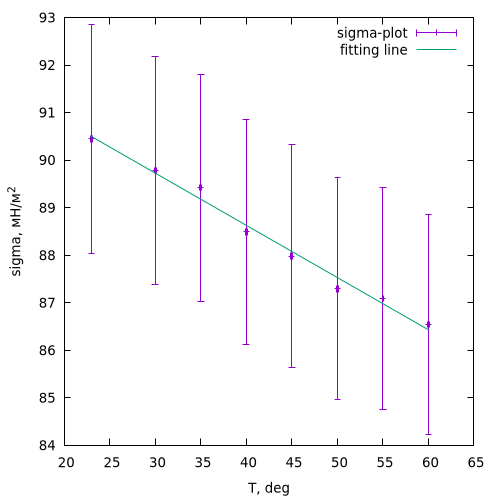
\includegraphics[width=0.90\textwidth]{plot0.png}
\end{center}
Из МНК получаются коэффициенты:
$$\sigma = (93.0\pm0.2) \text{мН}/\text{м}^2 - (110 \pm 5) \text{$\mu$Н}/(\text{м}^2\,^\circ C).$$
Понятно, что погрешности этих величин неправильные. Намного удобнее считать МНК графика температуры от давления:
\begin{center}
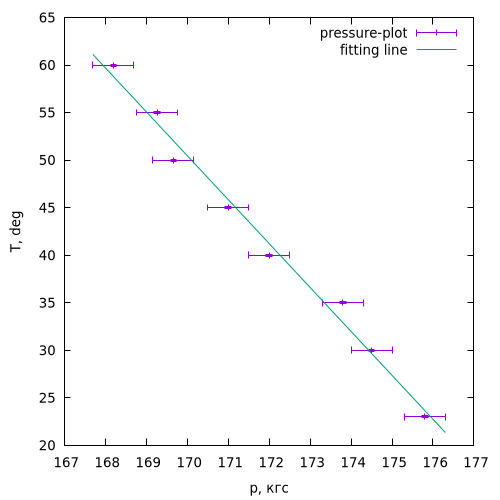
\includegraphics[width=0.90\textwidth]{plot1.png}
\end{center}
Так происходит из-за относительно высокого значения погрешности диаметра иголки.
Параметры этого графика:
$$T = (8.4\pm 0.4)\cdot10^2\,^\circ C - (4.6 \pm 0.2)\,\frac{^\circ C}{\text{кгс}}\cdot p.$$
Этой погрешности уже можно верить. Из нее получим
$$\frac{\delta \sigma}{\delta T} = \frac{d\sin(\alpha)}{4}\frac{\delta p}{\delta T} = (112\pm8)\frac{\text{$\mu$Н}}{\text{м}\,^\circ C}.$$
Также мы можем найти графики теплоты образования единицы поверхности жидкости $q$ и поверхнострую энергию $U$ площади $F$.
$$q = - T \frac{\delta \sigma}{\delta T}$$
$$U/F = \sigma - T \frac{\delta \sigma}{\delta T}$$
\begin{center}
\begin{tabular}{cc}
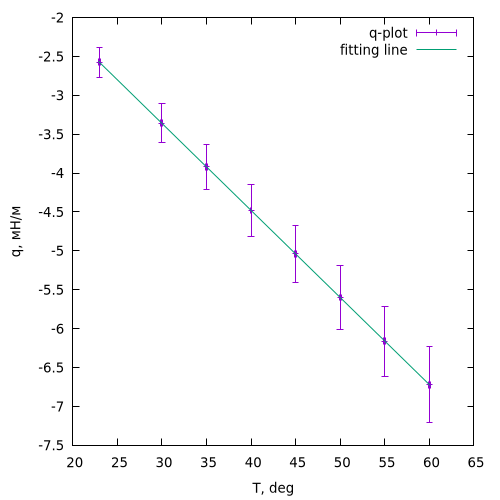
\includegraphics[width=0.48\textwidth]{plot2.png}&
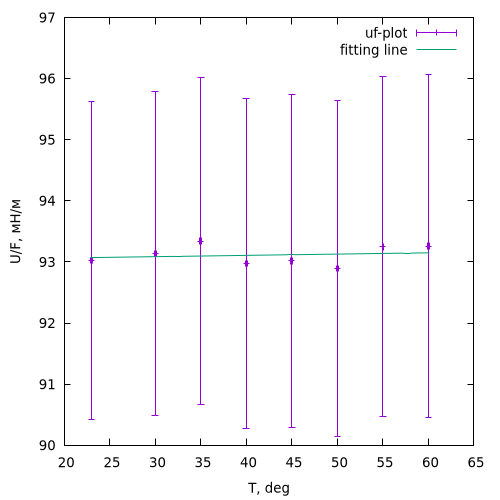
\includegraphics[width=0.48\textwidth]{plot3.png}\\
\end{tabular}
\end{center}

В этих графиках я брал полученное значение $\frac{\delta \sigma}{\delta T}$. Пересчет значений:
\begin{center}
\begin{tabular}{|c|c|c|c|c|c|}
\hline
$T\,^\circ C$&$\Delta T\,^\circ C$&$q,\,\frac{\text{мН}}{\text{м}}$&$\Delta q,\,\frac{\text{мН}}{\text{м}}$&$U/F,\,\frac{\text{мН}}{\text{м}}$&$\Delta (U/F),\,\frac{\text{мН}}{\text{м}}$\\
\hline
$23.0$&$0.1$&$-2.6$&$0.2$&$93$&$3$\\ \hline
$30.0$&$0.1$&$-3.4$&$0.3$&$93$&$3$\\ \hline
$35.0$&$0.1$&$-3.9$&$0.3$&$93$&$3$\\ \hline
$40.0$&$0.1$&$-4.5$&$0.3$&$93$&$3$\\ \hline
$45.0$&$0.1$&$-5.0$&$0.4$&$93$&$3$\\ \hline
$50.0$&$0.1$&$-5.6$&$0.4$&$93$&$3$\\ \hline
$55.0$&$0.1$&$-6.2$&$0.5$&$93$&$3$\\ \hline
$60.0$&$0.1$&$-6.7$&$0.5$&$93$&$3$\\ \hline
\end{tabular}.
\end{center}

\section*{Вывод}
Поверхностное натяжение линейно меняется от температуры, и мы смогли это пронаблюдать. Характеристики этой зависимости не совпали с табличными значениями, но не сильно (для задач на поверхностное натяжение) -- меньше, чем на 1 порядок. Главным источником погрешности в этом эксперименте являлась неточность измерения диаметра. Если бы я улучшал этот эксперимент, я бы двигался в направлении уменьшения этой погрешности -- например, давал бы табличную. Я научился измерять поверхностное натяжение границы жидкость-газ при помощи иглы и того факта, что пузырьки воздуха выходят из этой иглы только при определенном давлении, зависящем от $\sigma$.
\end{document}








\lipsum[1-4]
\begin{wrapfigure}{R}{5cm}
\centering
\includegraphics[width=0.20\textwidth]{rd.png}
\caption{1}
\end{wrapfigure}
\lipsum[1-6]


\begin{figure}[h]
\begin{center}$
\begin{array}{cccc}
\includegraphics[width=0.20\textwidth]{rd.png}&
\includegraphics[width=0.20\textwidth]{rd.png}&
\includegraphics[width=0.20\textwidth]{rd.png}&
\includegraphics[width=0.20\textwidth]{rd.png}\\
(1) & (2) & (3) & (4)
\end{array}$
\end{center}
\end{figure}